\raggedbottom
\section{Objetivos generales}
El objetivo general del trabajo es la elaboración de un prototipo funcional del videojuego EcoRescue, 
en el que los jugadores puedan acceder a niveles generados procedimentalmente, compuestos por un número
de 1-N biomas y de 1-3 problemas que vienen dados por la alteración seleccionada, cada bioma tiene 2 
alteraciones posibles, de los cuales se selecciona 1 aleatoriamente al iniciar un nivel. 
Posteriormente deberán poder informarse de estos, relacionar problemas y consecuencias y finalmente 
colocar máquinas en los biomas para restaurar los distintos problemas de cada alteracion.

El prototipo deberá tener interfaces funcionales que muestren la información de los niveles, biomas, alteraciones, problemas, consecuencias, máquinas y tutoriales (Figura \ref{fig:UI}). Los tutoriales vendrán dados por diálogos que saldrán del 
icono de un robot (Figura \ref{fig:robot}) que guiará al jugador durante su experiencia de juego.

\begin{figure}[H]
    \centering
      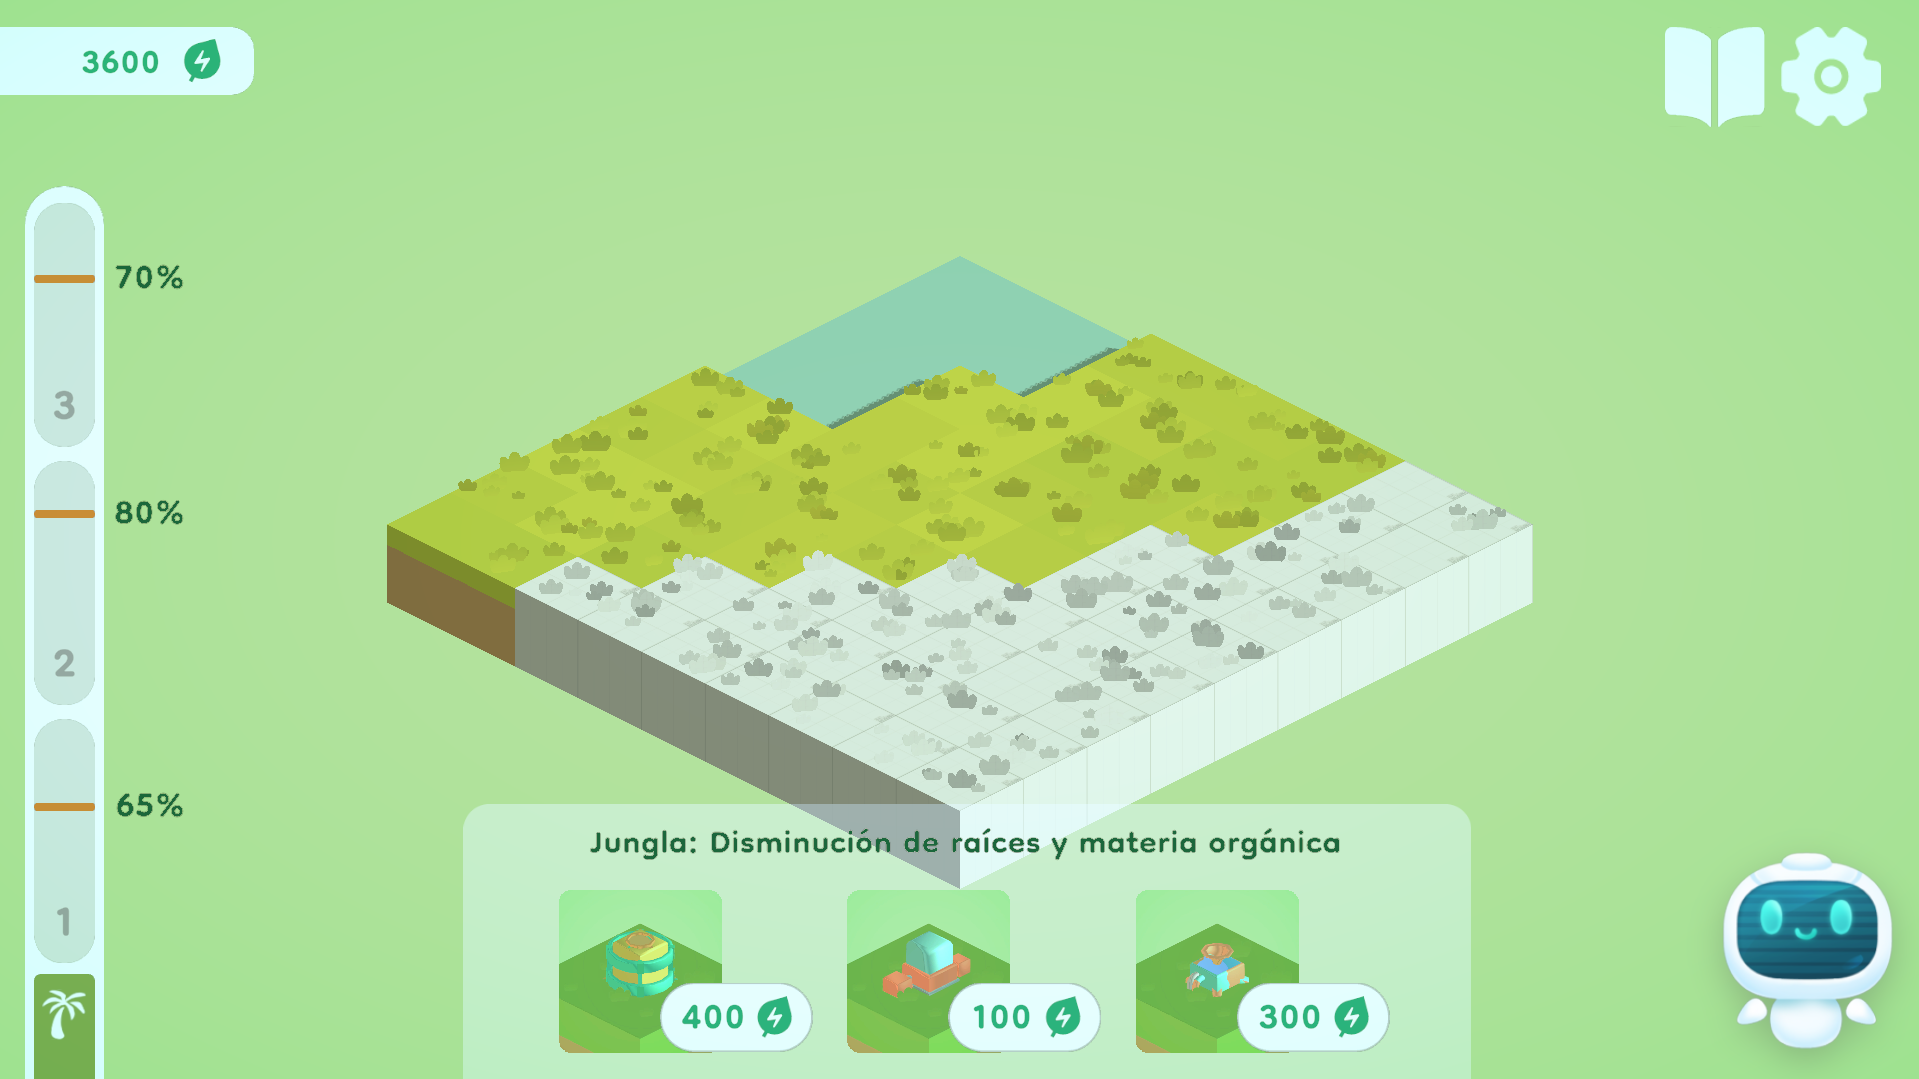
\includegraphics[width=350px,clip=true]{interfaz_restauracion.png}
    \caption{Interfaz general de EcoRescue}
    \label{fig:UI}
\end{figure}

\begin{figure}[H]
    \centering
      
\includegraphics[width=350px,clip=true]{convo_robot.png}
    \caption{Conversación de tutorial del robot}
    \label{fig:robot}
\end{figure}

El prototipo también deberá ser jugablemente disfrutable, esto implica desarrollar sistemas de control, sonido y animaciones que hagan que el juego sea vistoso y satisfactorio de jugar.

\subsection{Generación procedimental}

Una parte importante de EcoRescue es la facilidad de creación de contenido, para que desarrollar niveles sea más sencillo, el juego se ha enfocado desde un principio con la generación procedimental en mente, de forma que los niveles deberán generarse en base a algoritmia\cite{FastNoiseLite}, y cosas como las alteraciones en un nivel o el percentil al que se debe completar una fase deberán del mismo modo seguir un patrón procedimental.

\subsection{Herramientas del desarrollo}

De cara a la generación procedimental de niveles, el prototipo necesitará herramientas para que enlazar el gran volumen de contenido requerido por este enfoque de desarrollo con las estructuras internas del videojuego sea sencillo y mayormente automatizado. 

De esta forma, se requiere desarrollar un script que importe automáticamente todo el contenido (biomas, alteraciones, problemas, consecuencias, sprites, modelos...) desde un fichero de excel a un formato legible por el juego.

Además, también se requiere la creación de herramientas que permitan elegir de qué forma se quiere que se presente un nivel, incluyendo: personalización de las reglas de la generación procedimental de mapas, selección de Biomas por nivel y selección de Alteraciones por Bioma.

Además, el prototipo necesitará un sistema de generación de diálogos para que el robot de los tutoriales pueda comunicarse efectivamente con el jugador.

\subsection{Recogida de datos}

De cara a la medición de resultados, es necesario que el prototipo sea capaz de comunicarse con una base de datos para poder monitorizar las partidas de los jugadores y así poder interpretar sus movimientos. 
Esta comunicación con la base de datos debería recoger los datos básico  del usuario (nombre, edad...) (Figura \ref{fig:datos}) así como datos sobre su partida (máquinas colocadas, relaciones correctas, veces que ha perdido el nivel...).

\begin{figure}[H]
    \centering
      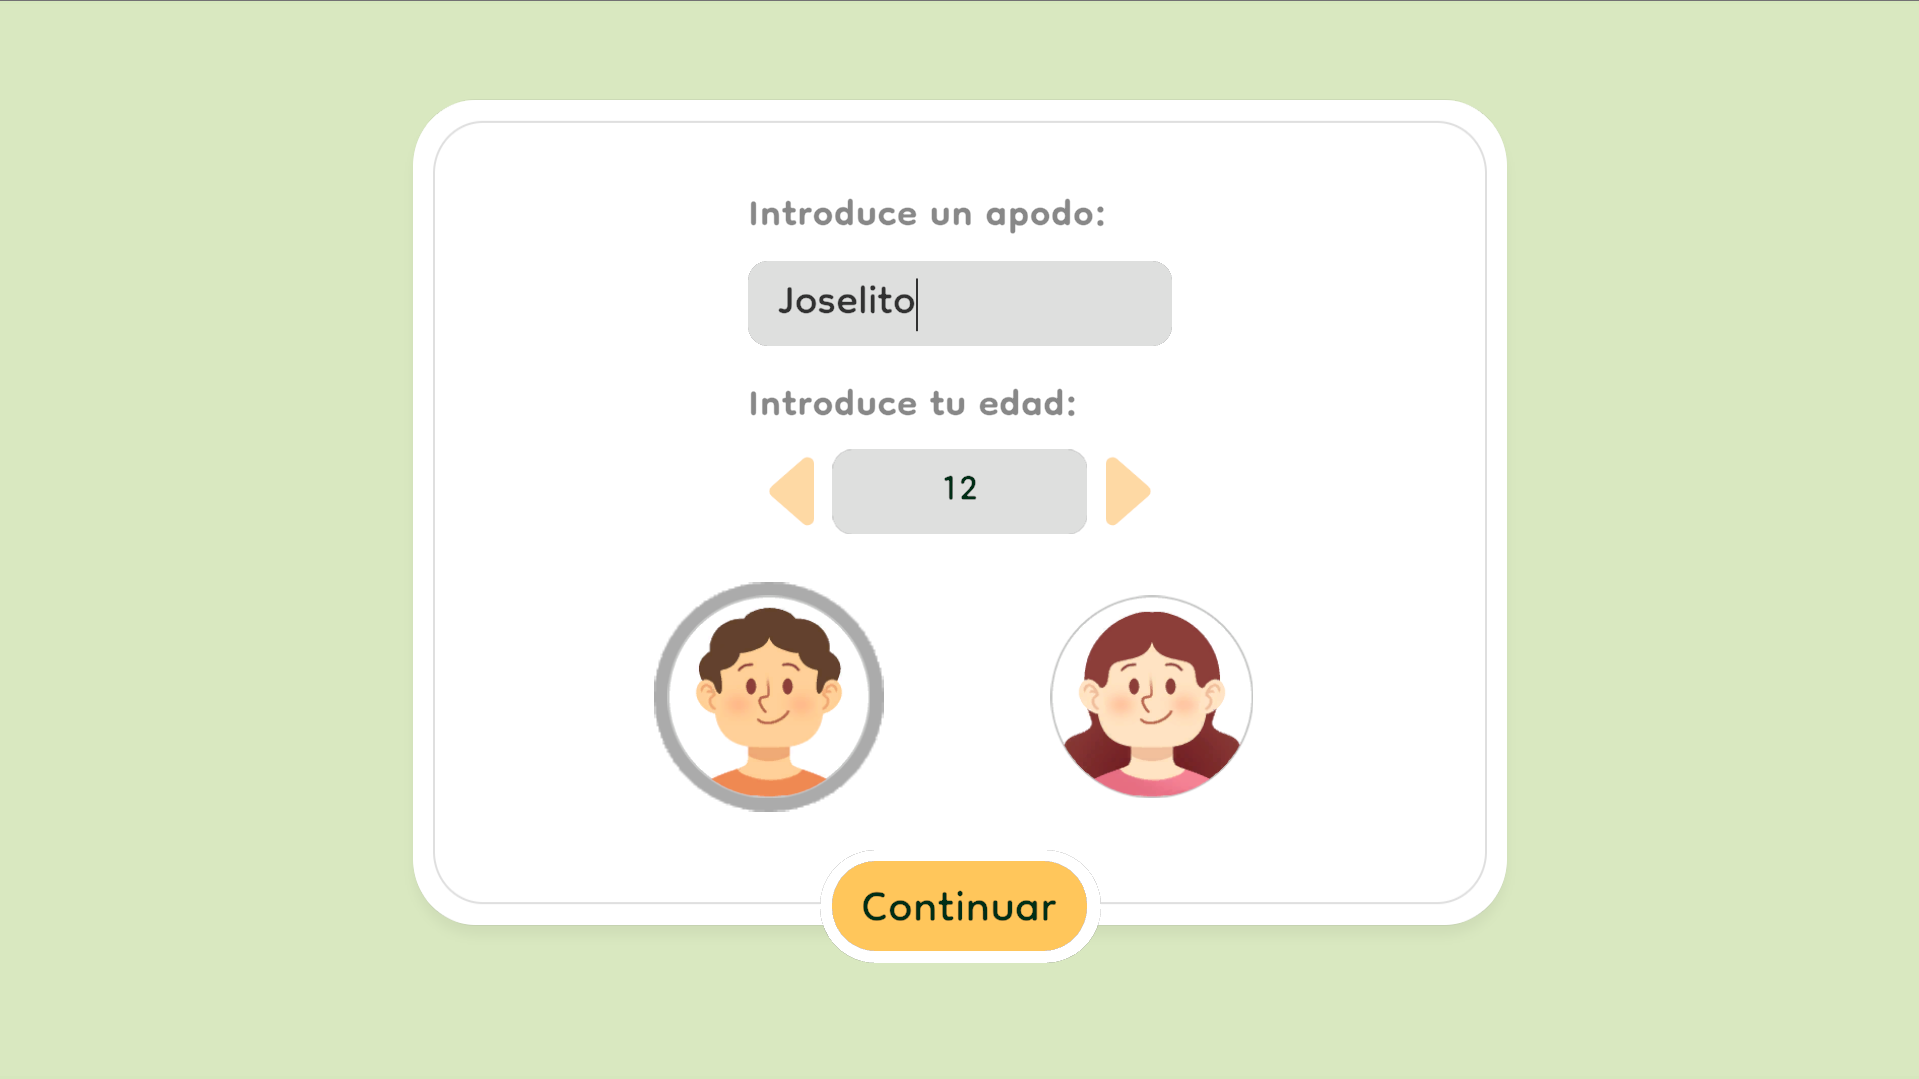
\includegraphics[width=350px,clip=true]{datos_pj.png}
    \caption{Pantalla de introducción de datos personales}
    \label{fig:datos}
\end{figure}

\subsection{Validación}

El objetivo más importante a nivel de proyecto es validar el prototipo frente a un grupo de alumnos de 1º de la ESO reales, con el objetivo de poder utilizar los datos de una encuesta así como los datos obtenidos en la base de datos para poder extraer conclusiones acerca de la efectividad del prototipo como herramienta didáctica para el desarrollo del PC, además de como herramienta divulgativa en lo referente a la restauración de ecosistemas.
Queda patente, pues, que los objetivos de la validación deben ser:
\begin{compactitem}
    \item Que el juego verdaderamente sirva para desarrolar el PC.
    \item Que el juego divulge información interesante acerca de la restauración de ecosistemas.
    \item Que el juego resulte una expriencia amena y divertida, a fin de que los alumnos disfruten del aprendizaje.
\end{compactitem} 

\section{Resumen de Objetivos}

En resumen, el el proyecto pretende:
\begin{enumerate}
    \item Desarrollar un juego completo y funcional que permita al jugador informarse sobre la restauración de ecosistemas y actuar en consecuencia.
    \item Desarrollar el PC del jugador en el aula.
    \item Desarrollar un juego que sea divertido y ameno.
    \item Desarrollar un juego con niveles generados procedimentalmente, además de herramientas que permitan crear contenido de forma eficiente para este.
    \item Recabar información sobre las partidas de los jugadores con el objetivo de interpretar sus movimientos y extraer conclusiones sobre la efectividad del prototipo.
\end{enumerate}